
%-------------------------------------------------------------------------------
%	CAPITOLO 23
%-------------------------------------------------------------------------------

\chapter{L'istrumento di divisione - tre paoli}

Questo capitolo è presente nell'indice, ma non vi è nei manoscritti. Probabilmente Mingazzi lo scrisse altrove ed è andato perduto. Non lo scopriremo mai.\\

Riporto in figura il capitoletto nell'indice.
 \begin{figure}[htb]
    \centering
    %\vspace{-0.7cm}
    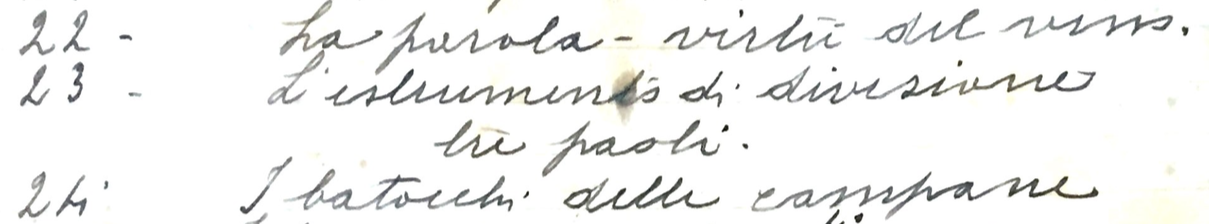
\includegraphics[width=\textwidth]{capitolo23}
    %\vspace{-0.3cm}
\end{figure}